\chapter{Hazard of Overfitting}
\lecture{13}{21 Oct.}{}

\begin{prev}
    A nonlinear feature transform \(\bm{\Phi}\) turns every linear model into a
    nonlinear one, at a price in \(\dvc\). The \(\bm{\Phi}_4\) boundary of
    \autoref{sec:transform-price} paid that price in full: zero \(\Ein\), and a
    boundary nobody believes. The advice was to start from the linear model,
    but the danger itself was only pointed at.
\end{prev}

This chapter opens topic~4, \emph{How Can Machines Learn Better?}, by naming
that danger and taking it apart. Overfitting turns out to be a \emph{move} to a
larger model that lowers \(\Ein\) but raises \(\Eout\). It is driven by small
data, noise and excessive model power, and also by a complicated target even
when there is no noise at all. That last effect is a second kind of noise,
\emph{deterministic} noise: the part of \(f\) that \(\mathcal{H}\) cannot
capture. The chapter ends with a first set of remedies that work on the data
themselves.

\section{What is Overfitting?}\label{sec:what-overfit}

\source{slides p.2--5}

\subsection{Bad Generalization}

The smallest example of things going wrong:

\begin{center}
    \begin{tikzpicture}
        \begin{axis}[ovfplot]
            \ovfFiveData
            \ovfFiveTarget
            \ovfFiveFit
            \legend{Data, Target, Fit}
        \end{axis}
    \end{tikzpicture}
\end{center}

\begin{itemize}
    \item The task is regression for \(x \in \mathbb{R}\), with only \(N = 5\)
        examples.
    \item The target \(f(x)\) is a 2nd order polynomial (the blue curve).
    \item Each label is \(y_n = f(x_n) + \) very small noise, so the five points
        sit almost exactly on the parabola.
    \item We learn by linear regression in \(\mathcal{Z}\)-space, with \(\bm{\Phi}
        = \) 4th order polynomial, \(\bm{\Phi}_4(x) = (1, x, x^2, x^3, x^4)\).
    \item That gives 5 weights for 5 examples. \(\mathrm{Z}\) is a square
        Vandermonde matrix, invertible because the \(x_n\) are distinct, so
        there is a unique solution passing all examples (the red curve), and
        \(\Ein(g) = 0\).
    \item To pass exactly through points that the noise has nudged off the
        parabola, the quartic must swing far from \(f\) in the wide gap between the
        leftmost point and the other four, where there is no data. \(\Eout(g)\) averages the error over all \(x\),
        so it is \textbf{huge}.
\end{itemize}

\begin{moral}
    Bad generalization: low \(\Ein\), high \(\Eout\).
\end{moral}

\subsection{Bad Generalization and Overfitting}

The VC picture of \autoref{sec:vc-interpret} says the same thing in general.
Moving right along the \(\dvc\) axis, \(\Ein\) falls while the model-complexity
term rises; \(\Eout\), bounded by their sum, is smallest at some
\(d_{\mathrm{VC}}^*\).

\begin{center}
    \vccurve
\end{center}

Three places on this curve get three names:
\begin{itemize}
    \item Taking \(\dvc = 1126\) for learning lands far to the right, where
        \((\Eout - \Ein)\) is large. This is \vocab{bad generalization}, a
        property of a single hypothesis set.
    \item Switching from \(\dvc = d_{\mathrm{VC}}^*\) to \(\dvc = 1126\)
        compares two sets: \(\Ein \downarrow\) but \(\Eout \uparrow\), because
        the gap grows faster than \(\Ein\) shrinks. This move is
        \vocab{overfitting}.
    \item Switching from \(\dvc = d_{\mathrm{VC}}^*\) to \(\dvc = 1\) goes the
        other way and makes both worse, \(\Ein \uparrow\) and \(\Eout
        \uparrow\). This is \vocab{underfitting}.
\end{itemize}
The quartic of the previous subsection is both: it generalizes badly, and it
is an overfit compared with the quadratic.

\begin{moral}
    Bad generalization: low \(\Ein\), high \(\Eout\);\\
    overfitting: low\textbf{er} \(\Ein\), high\textbf{er} \(\Eout\).
\end{moral}

\subsection{Cause of Overfitting: A Driving Analogy}

Fit the same five examples twice. On the left is a `good fit', a curve that
lies almost on top of \(f\); how to obtain it from the same 4th-order model is
the subject of the next chapter. On the right is the 4th-order interpolant from
before, the overfit.

\begin{center}
    \begin{tikzpicture}
        \begin{axis}[ovfplot, name=good,
            title={`good fit'}, title style={font=\small}]
            \ovfFiveData
            \ovfFiveTarget
            \ovfFiveGood
            \legend{Data, Target, Fit}
        \end{axis}
        \node at (6.15,1.5) {\(\Longrightarrow\)};
        \begin{axis}[ovfplot, at={(7.0cm,0)},
            title={\textbf{overfit}}, title style={font=\small}]
            \ovfFiveData
            \ovfFiveTarget
            \ovfFiveFit
            \legend{Data, Target, Fit}
        \end{axis}
    \end{tikzpicture}
\end{center}

What turns the left picture into the right one is easiest to see with an
analogy to driving.

\begin{center}
    \solidrules
    \begin{tabular}{c|c}
        \toprule
        learning & driving\\
        \midrule
        overfit & commit a car accident\\
        use excessive \(\dvc\) & `drive too fast'\\
        \textbf{noise} & bumpy road\\
        \textbf{limited data size \(N\)} & limited observations about road
        condition\\
        \bottomrule
    \end{tabular}
\end{center}

Speed alone does not cause an accident: the accident comes from speed on a
bumpy road that the driver cannot see well. In the pictures, the 4th-order
model is the speed. The noise and the mere five examples are the road. The
good fit drives the same road slowly and stays on \(f\). Excessive
\(\dvc\) was already the subject of the VC curve. The other two causes are new.

\begin{question}
    How does \textbf{noise} \& \textbf{data size} affect overfitting?
\end{question}

\begin{exercise}[Fun Time]
    Based on our discussion, for data of fixed size, which of the following
    situation is relatively of the lowest risk of overfitting?
    \begin{enumerate}[(1)]
        \item small noise, fitting from small \(\dvc\) to median \(\dvc\);
        \item small noise, fitting from small \(\dvc\) to large \(\dvc\);
        \item large noise, fitting from small \(\dvc\) to median \(\dvc\);
        \item large noise, fitting from small \(\dvc\) to large \(\dvc\).
    \end{enumerate}
\end{exercise}

\begin{proof}[Reference Answer]
    (1). Two causes of overfitting are noise and excessive \(\dvc\). So if
    both are relatively `under control', the risk of overfitting is smaller.
\end{proof}

\section{The Role of Noise and Data Size}\label{sec:noise-data-size}

\source{slides p.6--11}

\subsection{Case Study}

Take two data sets of \(N = 15\) examples each. On the left the target is a
10th-order polynomial and the labels carry noise. On the
right the target is a 50th-order polynomial, but the labels are
noiseless: every point lies exactly on \(f\).

\begin{center}
    \begin{tikzpicture}
        \begin{axis}[ovfplot,
            title={10-th order target function \(+\) \textbf{noise}},
            title style={font=\small}]
            \ovfTenData
            \ovfTenTarget
            \legend{Data, Target}
        \end{axis}
        \begin{axis}[ovfplot, at={(7.2cm,0)},
            title={50-th order target function \textbf{noiselessly}},
            title style={font=\small}]
            \ovfFiftyData
            \ovfFiftyTarget
            \legend{Data, Target}
        \end{axis}
    \end{tikzpicture}
\end{center}

On each, compare two hypothesis sets. \(\mathcal{H}_Q\) is the polynomials of
order \(Q\), i.e.\ linear regression after \(\bm{\Phi}_Q\), and \(g_Q\) is its
least-squares best on the 15 examples.

\begin{question}
    Overfitting from best \(g_2 \in \mathcal{H}_2\) to best \(g_{10} \in
    \mathcal{H}_{10}\)?
\end{question}

\begin{center}
    \begin{tikzpicture}
        \begin{axis}[ovfplot,
            title={10-th order target function \(+\) \textbf{noise}},
            title style={font=\small}]
            \ovfTenData
            \ovfTenFitTwo
            \ovfTenFitTen
            \legend{Data, 2nd Order Fit, 10th Order Fit}
        \end{axis}
        \begin{axis}[ovfplot, at={(7.2cm,0)},
            title={50-th order target function \textbf{noiselessly}},
            title style={font=\small}]
            \ovfFiftyData
            \ovfFiftyFitTwo
            \ovfFiftyFitTen
            \legend{Data, 2nd Order Fit, 10th Order Fit}
        \end{axis}
    \end{tikzpicture}
\end{center}

In both plots the red 10th-order fit passes closer to the points than the green
parabola, so its \(\Ein\) is lower. Between and beyond the points, most of all
near \(\pm 1\), it swings wildly: 11 weights fitted to 15 points leave little
to keep it in place where there is no data. The table puts numbers on this.

\begin{center}
    \begin{tabular}{l|cc}
        \multicolumn{3}{c}{10-th order \(+\) noise}\\[2pt]
        & \(g_2 \in \mathcal{H}_2\) & \(g_{10} \in \mathcal{H}_{10}\)\\
        \hline
        \(\Ein\) & 0.050 & 0.034\\
        \(\Eout\) & 0.127 & \textbf{9.00}
    \end{tabular}
    \hspace{1.2cm}
    \begin{tabular}{l|cc}
        \multicolumn{3}{c}{50-th order, noiseless}\\[2pt]
        & \(g_2 \in \mathcal{H}_2\) & \(g_{10} \in \mathcal{H}_{10}\)\\
        \hline
        \(\Ein\) & 0.029 & 0.00001\\
        \(\Eout\) & 0.120 & \textbf{7680}
    \end{tabular}
\end{center}

\(\Ein\) improves a little in both cases, while \(\Eout\) grows by a factor of
about \(70\) on the left and \(6 \times 10^4\) on the right. Both moves are
overfitting in the sense of \autoref{sec:what-overfit}.

\begin{moral}
    Overfitting from \(g_2\) to \(g_{10}\)? \textbf{both yes!}
\end{moral}

\subsection{Irony of Two Learners}

\begin{center}
    \begin{tikzpicture}
        \begin{axis}[ovfplot]
            \ovfTenData
            \ovfTenFitTwo
            \ovfTenFitTen
            \legend{Data, 2nd Order Fit, 10th Order Fit}
        \end{axis}
        \begin{axis}[ovfplot, at={(7.2cm,0)}]
            \ovfTenData
            \ovfTenTarget
            \legend{Data, Target}
        \end{axis}
    \end{tikzpicture}
\end{center}

Name the two choices after two learners.
\begin{itemize}
    \item Learner \emph{Overfit} (\(O\)) picks \(g_{10} \in
        \mathcal{H}_{10}\).
    \item Learner \emph{Restrict} (\(R\)) picks \(g_2 \in \mathcal{H}_2\).
    \item Suppose both know that the target is 10th order. Then \(O\) seems to
        have the right model, since \(f \in \mathcal{H}_{10}\), while \(R\)
        `gives up' the ability to fit \(f\) at all.
\end{itemize}
Yet the left plot shows the green parabola following the overall trend of the
target and the red curve oscillating far from it. \(\mathcal{H}_{10}\) does
contain a hypothesis with \(\Eout = \sigma^2\), the best possible, but \(O\)
has to find it from 15 noisy examples, and 11 weights estimated from 15 points
mostly follow the noise. \(R\) estimates only 3 weights from the same points,
which is reliable.

\begin{moral}
    But \(R\) \textbf{wins in \(\Eout\)} a lot!\\
    Philosophy: concession for advantage? :-)
\end{moral}

\subsection{Learning Curves Revisited}

\begin{center}
    \begin{tikzpicture}
        \begin{groupplot}[group style={group size=2 by 1,
                horizontal sep=1.6cm},
            width=6.0cm, height=4.6cm, xmin=0, xmax=60, ymin=0, ymax=2.6,
            axis lines=left, xtick=\empty, ytick=\empty,
            xlabel={Number of Data Points, \(N\)},
            ylabel={Expected Error}, label style={font=\small},
            title style={font=\small}]
            \nextgroupplot[title={\(\mathcal{H}_2\)}]
            \fill[black!20] (axis cs:0,0) rectangle (axis cs:29,2.6);
            \addplot[black, thin, domain=0:60] {1.25};
            \addplot[red!85!black, thick, domain=3.5:60, samples=80]
                {1.25*(1 + 3/x)};
            \addplot[blue!85!black, thick, domain=3:60, samples=80]
                {1.25*(1 - 3/x)};
            \node[text=red!85!black, font=\small] at (axis cs:45,1.6)
                {\(\Eout\)};
            \node[text=blue!85!black, font=\small] at (axis cs:45,0.95)
                {\(\Ein\)};
            \nextgroupplot[title={\(\mathcal{H}_{10}\)}]
            \fill[black!20] (axis cs:0,0) rectangle (axis cs:29,2.6);
            \addplot[black, thin, domain=0:60] {1};
            \addplot[red!85!black, thick, domain=11:60, samples=80]
                {1 + 11/x};
            \addplot[blue!85!black, thick, domain=11:60, samples=80]
                {1 - 11/x};
            \node[text=red!85!black, font=\small] at (axis cs:45,1.48)
                {\(\Eout\)};
            \node[text=blue!85!black, font=\small] at (axis cs:45,0.55)
                {\(\Ein\)};
        \end{groupplot}
    \end{tikzpicture}
\end{center}

These are the learning curves of \autoref{sec:learning-curve}, drawn for
\(\mathcal{H}_2\) and \(\mathcal{H}_{10}\): expected \(\Ein\) (blue) and
\(\Eout\) (red) against \(N\). Both approach the black line, the error that
remains with unlimited data. That line is lower for \(\mathcal{H}_{10}\), which
contains the target, than for \(\mathcal{H}_2\), which does not.
\begin{itemize}
    \item \(\mathcal{H}_{10}\) has the lower \(\Eout\) when \(N \to \infty\),
        but a much larger generalization error (the gap between red and blue)
        for small \(N\), because it has more weights to estimate.
    \item In the {\setlength{\fboxsep}{1.5pt}\colorbox{black!20}{gray area}},
        \(O\) overfits: compared with \(\mathcal{H}_2\), its \(\Ein\) is lower
        but its \(\Eout\) is higher. The case study, with \(N = 15\), sits in
        this region.
\end{itemize}

\begin{moral}
    \(R\) always \textbf{wins in \(\Eout\)} if \(N\) small!
\end{moral}

\subsection{The `No Noise' Case}

\begin{center}
    \begin{tikzpicture}
        \begin{axis}[ovfplot]
            \ovfFiftyData
            \ovfFiftyFitTwo
            \ovfFiftyFitTen
            \legend{Data, 2nd Order Fit, 10th Order Fit}
        \end{axis}
        \begin{axis}[ovfplot, at={(7.2cm,0)}]
            \ovfFiftyData
            \ovfFiftyTarget
            \legend{Data, Target}
        \end{axis}
    \end{tikzpicture}
\end{center}

Now take the right-hand data set of the case study.
\begin{itemize}
    \item Learner \emph{Overfit} (\(O\)) again picks \(g_{10} \in
        \mathcal{H}_{10}\).
    \item Learner \emph{Restrict} (\(R\)) again picks \(g_2 \in
        \mathcal{H}_2\).
    \item This time both know that there is no noise, so \(O\) can argue that
        every point is exact and there is nothing to overfit. Still, \(R\)
        wins: the red fit chases the points and swings away from the target
        between them.
\end{itemize}

\begin{question}
    Is there really \textbf{no noise}?
\end{question}

\begin{moral}
    `Target complexity' acts like noise.
\end{moral}

Neither \(\mathcal{H}_2\) nor \(\mathcal{H}_{10}\) contains the 50th-order
target, so no hypothesis can follow the fast wiggles of \(f\). Seen from inside
\(\mathcal{H}_{10}\), the labels \(y_n\) deviate from the best hypothesis in a
way nothing can explain. That is exactly what noise did on the left of the
case study. \(\mathcal{H}_{10}\), with more weights, bends further to fit those
deviations, and pays for it the same way.

\begin{exercise}[Fun Time]
    When having limited data, in which of the following case would learner
    \(R\) perform better than learner \(O\)?
    \begin{enumerate}[(1)]
        \item limited data from a 10-th order target function with some noise;
        \item limited data from a 1126-th order target function with no noise;
        \item limited data from a 1126-th order target function with some
            noise;
        \item all of the above.
    \end{enumerate}
\end{exercise}

\begin{proof}[Reference Answer]
    (4). We discussed about (1) and (2), but you shall be able to `generalize'
    :-) that \(R\) also wins in the more difficult case of (3).
\end{proof}

\section{Deterministic Noise}\label{sec:det-noise}

\source{slides p.12--17}

\subsection{A Detailed Experiment}\label{sec:detailed-experiment}

The case study had two data sets. To see \emph{how much} noise and target
complexity it takes, the same comparison is repeated over a whole grid of
settings.

\begin{center}
    \begin{minipage}[c]{0.5\textwidth}
        \[
            y = f(x) + \epsilon \sim \text{Gaussian} \Biggl(
            \underbrace{\sum_{q=0}^{Q_f} \alpha_q x^q}_{f(x)}, \sigma^2
            \Biggr)
        \]
    \end{minipage}%
    \begin{minipage}[c]{0.45\textwidth}
        \centering
        \begin{tikzpicture}
            \begin{axis}[ovfplot]
                \ovfTenData
                \ovfTenTarget
                \legend{Data, Target}
            \end{axis}
        \end{tikzpicture}
    \end{minipage}
\end{center}

Each label is \(f(x)\) plus Gaussian noise, and the experiment has three
knobs:
\begin{itemize}
    \item Gaussian iid noise \(\epsilon\) with level \(\sigma^2\);
    \item a target \(f\) drawn from some `uniform' distribution with
        complexity level \(Q_f\), the order of the polynomial;
    \item the data size \(N\).
\end{itemize}
The plot shows one draw, with \(Q_f = 10\) and \(N = 15\).

`Uniform' means that the coefficients are drawn at random and rescaled so that
every \(f\) has the same overall size. A given \(\sigma^2\) then means the same
amount of noise relative to the signal, whatever \(Q_f\) is.

\begin{question}
    Goal: `overfit level' for different \((N, \sigma^2)\) and \((N, Q_f)\)?
\end{question}

\subsection{The Overfit Measure}

\begin{center}
    \begin{tikzpicture}
        \begin{axis}[ovfplot]
            \ovfTenData
            \ovfTenFitTwo
            \ovfTenFitTen
            \legend{Data, 2nd Order Fit, 10th Order Fit}
        \end{axis}
        \begin{axis}[ovfplot, at={(7.2cm,0)}]
            \ovfTenData
            \ovfTenTarget
            \legend{Data, Target}
        \end{axis}
    \end{tikzpicture}
\end{center}

For every setting, draw a data set and fit it twice, exactly as in the case
study.
\begin{itemize}
    \item \(g_2 \in \mathcal{H}_2\) is the least-squares best quadratic.
    \item \(g_{10} \in \mathcal{H}_{10}\) is the least-squares best 10th-order
        polynomial.
    \item \(\Ein(g_{10}) \le \Ein(g_2)\) holds for sure, by
        \autoref{prop:nested}: \(\mathcal{H}_2 \subset \mathcal{H}_{10}\), and
        the minimum over a larger set is no larger.
\end{itemize}
So half of overfitting, \(\Ein \downarrow\), is automatic, and whether the move
overfits depends only on \(\Eout\).

\begin{moral}
    Overfit measure \(\Eout(g_{10}) - \Eout(g_2)\).
\end{moral}

Positive means the move to \(\mathcal{H}_{10}\) overfitted; negative means it
was worth it.

\subsection{The Results}

\begin{center}
    \begin{adjustbox}{max width=\textwidth}
        \begin{tabular}{cc}
            impact of \(\sigma^2\) versus \(N\) & impact of \(Q_f\) versus
            \(N\)\\[2pt]
            \overfitmap{overfit_noise_level.png}{-0.005}{2.505}%
                {Noise Level, \(\sigma^2\)}{0,1,2}
            &
            \overfitmap{overfit_target_complexity.png}{-0.5}{100.5}%
                {Target Complexity, \(Q_f\)}{0,25,50,75,100}\\[2pt]
            fixed \(Q_f = 20\) & fixed \(\sigma^2 = 0.1\)
        \end{tabular}
    \end{adjustbox}
\end{center}

Each pixel is one setting, coloured by the overfit measure clipped to
\([-0.2, 0.2]\). Dark red is serious overfitting; dark blue means
\(\mathcal{H}_{10}\) clearly won.

The left map varies the noise \(\sigma^2\) against \(N\), with \(Q_f = 20\)
fixed. Red fills the upper left, where examples are few and noise is high. Its
edge is a rising diagonal: the more noise, the more examples are needed before
\(\mathcal{H}_{10}\) is safe.

The right map varies the target complexity \(Q_f\) against \(N\), with
\(\sigma^2 = 0.1\) fixed and small. Above \(Q_f \approx 10\), red still fills
the left side and widens as \(Q_f\) grows, although the noise never changes.
The thin band at the bottom depends on which sets contain \(f\). For \(Q_f
\le 2\) both do, so the extra weights of \(\mathcal{H}_{10}\) only fit noise
and the measure is positive. For \(3 \le Q_f \le 10\) only \(\mathcal{H}_{10}\)
does, so it wins (dark blue). Above \(10\) neither does, and the red returns.

\begin{center}
    \textbf{ring a bell? :-)}\\[4pt]
    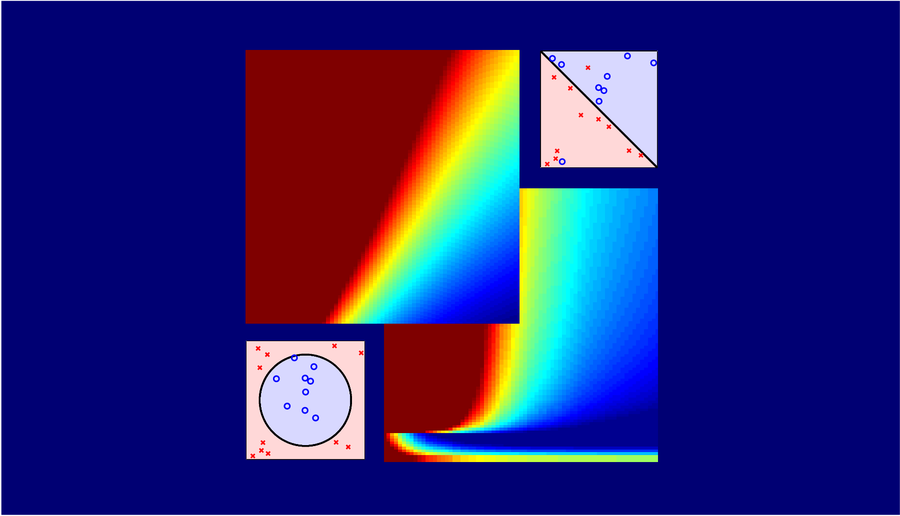
\includegraphics[width=4.2cm]{Figures/course_logo.png}
\end{center}

This is the picture on the title slide of every handout, the course's logo. It
is made of these two maps together with the linear-separable and
circular-separable data sets of \autoref{sec:quad-hyp}.

\subsection{Impact of Noise and Data Size}

\begin{center}
    \begin{adjustbox}{max width=\textwidth}
        \begin{tabular}{cc}
            impact of \(\sigma^2\) versus \(N\): & impact of \(Q_f\) versus
            \(N\):\\
            \textbf{stochastic noise} & \textbf{deterministic noise}\\[2pt]
            \overfitmap{overfit_noise_level.png}{-0.005}{2.505}%
                {Noise Level, \(\sigma^2\)}{0,1,2}
            &
            \overfitmap{overfit_target_complexity.png}{-0.5}{100.5}%
                {Target Complexity, \(Q_f\)}{0,25,50,75,100}
        \end{tabular}
    \end{adjustbox}
\end{center}

These are the same two maps. The new titles name the quantity on each vertical
axis.
\begin{itemize}
    \item On the left, the vertical axis \(\sigma^2\) is the level of the
        \vocab{stochastic noise}: the noise \(\epsilon\) of \autoref{sec:noise},
        drawn at random for each example. Moving up the map means more
        stochastic noise.
    \item On the right, the vertical axis \(Q_f\) measures the
        \textbf{deterministic noise}. \(\sigma^2\) is fixed here, so the only
        thing that changes is the target complexity. A more complex \(f\)
        leaves more of itself outside \(\mathcal{H}_2\) and \(\mathcal{H}_{10}\),
        and that part acts as noise. Moving up the map means more
        deterministic noise, which the next subsection defines.
\end{itemize}
Read this way, the two maps say the same thing: going up (more noise of either
kind) or left (fewer examples) makes overfitting worse. Collecting everything
so far:

\begin{center}
    four reasons of serious overfitting:\quad
    \begin{tabular}{rl}
        data size \(N\) \(\downarrow\) & overfit \(\uparrow\)\\
        \textbf{stochastic} noise \(\uparrow\) & overfit \(\uparrow\)\\
        \textbf{deterministic} noise \(\uparrow\) & overfit \(\uparrow\)\\
        excessive power \(\uparrow\) & overfit \(\uparrow\)
    \end{tabular}
\end{center}

The first three are read off the two maps. The fourth, \emph{excessive
power}, means a hypothesis set more flexible (larger \(\dvc\)) than the data
can support. It is the `use excessive \(\dvc\)', or `drive too fast', of the
driving analogy. In this experiment it is the switch from \(\mathcal{H}_2\) to
\(\mathcal{H}_{10}\), which is what every pixel measures. The 11 weights of
\(\mathcal{H}_{10}\) give it the power to follow noise that the 3 weights of
\(\mathcal{H}_2\) cannot. The more power beyond what is needed, the more
overfitting. Real problems usually have little data and some noise, and the
target is rarely simple, so all four are common.

\begin{moral}
    Overfitting `easily' happens.
\end{moral}

\subsection{Deterministic Noise}

Why does target complexity act like noise? In the picture, \(f\) is a wiggly
target, \(h^*\) is the best hypothesis in a simpler \(\mathcal{H}\) (closest to
\(f\) in squared error), and the gray area between them is what \(\mathcal{H}\)
can never reach.

\begin{center}
    \begin{tikzpicture}
        \begin{axis}[ovfplot, width=7.5cm, height=5.2cm]
            \ovfDetF
            \ovfDetHstar
            \addplot[detnoise] fill between[of=detf and dethstar];
            \node[text=blue!85!black, font=\small] at (axis cs:-0.72,0.13)
                {\(f\)};
            \node[text=red!85!black, font=\small] at (axis cs:0.1,0.93)
                {\(h^*\)};
        \end{axis}
    \end{tikzpicture}
\end{center}

\begin{itemize}
    \item If \(f \notin \mathcal{H}\), something of \(f\) cannot be captured by
        \(\mathcal{H}\).
    \item The \vocab{deterministic noise} is the difference between the best
        \(h^* \in \mathcal{H}\) and \(f\): the gray area.
    \item To a learner using \(\mathcal{H}\), it acts like `stochastic noise'.
        That is not new to CS: a pseudo-random generator outputs a fixed
        function of its seed, yet the output looks random to anyone who
        cannot model that function.
    \item It differs from stochastic noise in two ways.
        \begin{itemize}
            \item It depends on \(\mathcal{H}\): a larger set gets closer to
                \(f\) and leaves less of it.
            \item It is fixed for a given \(\bm{x}\): the same \(x_n\) always
                carries the same \(f(x_n) - h^*(x_n)\), whereas \(\epsilon\) is
                redrawn for each example.
        \end{itemize}
\end{itemize}
For every hypothesis in \(\mathcal{H}\), this gap costs about as much as
stochastic noise of the same size would. That is why \(\mathcal{H}_2\)'s black
line in the learning curves sits higher. The philosophy below is the same idea
applied to people: a target too complicated for what a kid can grasp only looks
like noise to them.

\begin{remark}
    `Deterministic noise \(\uparrow\)' in \autoref{sec:det-noise} (the right map
    and the table) means the \emph{target} getting more complex, with
    \(\mathcal{H}\) fixed. It does not mean the hypothesis set getting more
    complex. Making \(\mathcal{H}\) more complex goes the other way: \(h^*\)
    gets closer to \(f\), so the deterministic noise drops (the first
    difference above). It also adds power, though, and with little data the
    extra power costs more than the smaller deterministic noise saves, so a
    larger \(\mathcal{H}\) can still overfit.
\end{remark}

\begin{moral}
    Philosophy: when teaching a kid, perhaps better not to use examples from a
    complicated target function? :-)
\end{moral}

The exercise below asks for the deterministic noise point by point. For each
\(x\), the \vocab{level of deterministic noise} at \(x\) is the size of the gap
there,
\[
    \abs{f(x) - h^*(x)} .
\]

\begin{exercise}[Fun Time]
    Consider the target function being \(\sin(1126x)\) for \(x \in [0, 2\pi]\).
    When \(x\) is uniformly sampled from the range, and we use all possible
    linear hypotheses \(h(x) = \bm{w}^\top \bm{x}\) to approximate the target
    function with respect to the squared error, what is the level of
    deterministic noise for each \(x\)?
    \begin{enumerate}[(1)]
        \item \(\abs{\sin(1126x)}\);
        \item \(\abs{\sin(1126x) - x}\);
        \item \(\abs{\sin(1126x) + x}\);
        \item \(\abs{\sin(1126x) - 1126x}\).
    \end{enumerate}
\end{exercise}

\begin{proof}[Reference Answer]
    (1). You can try a few different \(\bm{w}\) and convince yourself that the
    best hypothesis \(h^*\) is \(h^*(x) = 0\). The deterministic noise is the
    difference between \(f\) and \(h^*\).
\end{proof}

With \(h^* \approx 0\), the level at \(x\) is \(\abs{\sin(1126x) - 0} =
\abs{\sin(1126x)}\). A line cannot follow the \(1126/\pi \approx 358\) full periods of
\(\sin(1126x)\) on \([0, 2\pi]\), so the best it can do is stay near their
average, \(0\).

\section{Dealing with Overfitting}\label{sec:deal-overfit}

\source{slides p.18--21}

\subsection{Driving Analogy Revisited}

\begin{center}
    \solidrules
    \begin{tabular}{c|c}
        \toprule
        learning & driving\\
        \midrule
        overfit & commit a car accident\\
        use excessive \(\dvc\) & `drive too fast'\\
        noise & bumpy road\\
        limited data size \(N\) & limited observations about road condition\\
        \midrule[\heavyrulewidth]
        \textbf{start from simple model} & drive slowly\\
        \textbf{data cleaning/pruning} & use more accurate road information\\
        \textbf{data hinting} & exploit more road information\\
        \textbf{regularization} & put the brakes\\
        \textbf{validation} & monitor the dashboard\\
        \bottomrule
    \end{tabular}
\end{center}

The lower half of the table extends the analogy to remedies, each aimed at a
cause in the upper half. Starting from a simple model is driving slowly: it
keeps \(\dvc\) small, the `linear model first' of \autoref{sec:structured-H}.
Data cleaning/pruning gives more accurate road information, i.e.\ less noise.
Data hinting exploits more road information, i.e.\ more data. Both are
treated in the rest of this section. Regularization puts on the brakes, and
validation watches the dashboard; they take the next chapters.

\begin{moral}
    All very \textbf{practical} techniques to combat overfitting.
\end{moral}

\subsection{Data Cleaning/Pruning}

\begin{center}
    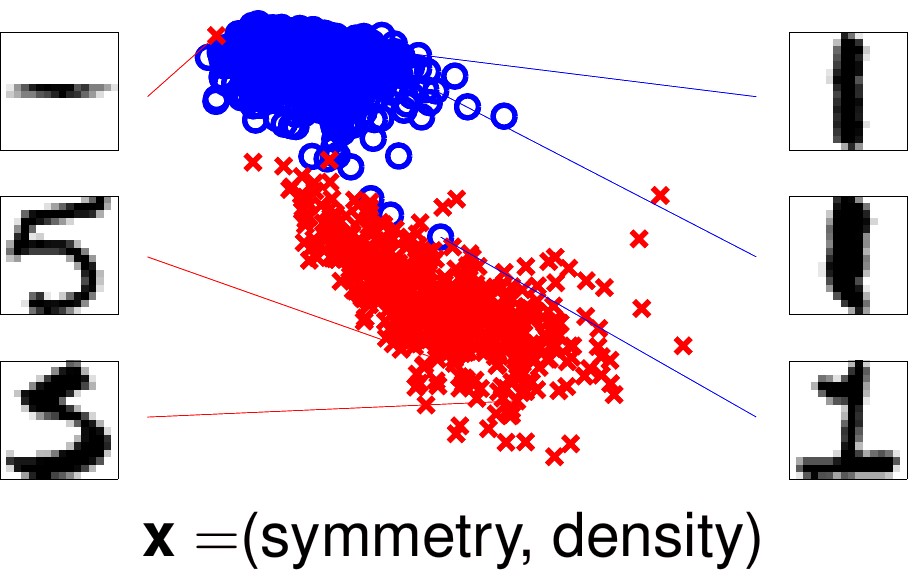
\includegraphics[width=0.55\textwidth]{Figures/digit_features.png}
\end{center}

This is the `1' (\(\circ\)) versus `5' (\(\times\)) data of
\autoref{def:raw}, each digit reduced to its symmetry and density. One
\(\times\) sits at the very top, inside the cloud of \(\circ\)'s. It is labelled
`5', but its image, the top-left thumbnail, is a short horizontal stroke: a
symmetric, light image, with exactly the features of a `1'. To the learner it
is noise.

\begin{itemize}
    \item We might `detect' the outlier 5 at the top
        \begin{itemize}
            \item because it is too close to other \(\circ\), or too far from
                other \(\times\);
            \item because it is wrong by the current classifier;
            \item or by other rules (\ldots).
        \end{itemize}
    \item Possible action 1 is to correct its label (\vocab{data cleaning}).
    \item Possible action 2 is to remove the example (\vocab{data pruning}).
\end{itemize}
Either action lowers the noise the learner sees. Both depend on the detection,
though, and the same rules also flag examples that are correct but unusual.
Removing those leaves a less representative data set.

\begin{moral}
    Possibly helps, but \textbf{effect varies}.
\end{moral}

\subsection{Data Hinting}

\begin{center}
    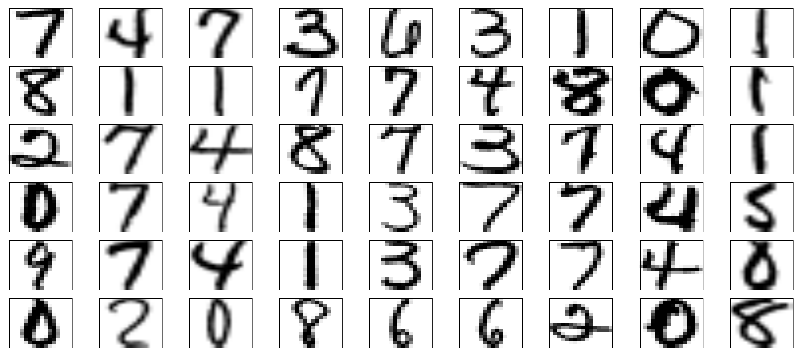
\includegraphics[width=0.55\textwidth]{Figures/digits_grid.png}
\end{center}

The grid shows handwritten digits from the training data.
\begin{itemize}
    \item Slightly shifted or rotated digits carry the same meaning: a `7'
        moved by one pixel or tilted a few degrees is still a `7'.
    \item The possible action is to add \vocab{virtual examples} by shifting or
        rotating the given digits, keeping their labels (\vocab{data
        hinting}).
\end{itemize}
This turns prior knowledge about \(f\) into data, making \(N\) larger without
collecting anything new.

\begin{moral}
    Possibly helps, but \textbf{watch out} --- virtual example not
    \(\overset{\mathrm{iid}}{\sim} P(\bm{x}, y)\)!
\end{moral}

The catch is that the Hoeffding and VC guarantees of the earlier chapters
assume examples drawn iid from the same \(P\) that \(\Eout\) is measured on.
Virtual examples are copies of existing ones, so they are not independent of
them and not drawn from \(P\). A rotation large enough to turn a `6' into a
`9' would even teach the wrong label.

\begin{exercise}[Fun Time]
    Assume we know that \(f(x)\) is symmetric for some 1D regression
    application. That is, \(f(x) = f(-x)\). One possibility of using the
    knowledge is to consider symmetric hypotheses only. On the other hand, you
    can also generate virtual examples from the original data \(\{(x_n,
    y_n)\}\) as hints. What virtual examples suit your needs best?
    \begin{enumerate}[(1)]
        \item \(\{(x_n, -y_n)\}\);
        \item \(\{(-x_n, -y_n)\}\);
        \item \(\{(-x_n, y_n)\}\);
        \item \(\{(2x_n, 2y_n)\}\).
    \end{enumerate}
\end{exercise}

\begin{proof}[Reference Answer]
    (3). We want the virtual examples to encode the invariance when \(x \to
    -x\). Since \(f(-x_n) = f(x_n)\), the label \(y_n\) is just as valid at
    \(-x_n\).
\end{proof}

\hrulebar

\subsection*{Summary}

\begin{description}
    \item[What is Overfitting?] lower \(\Ein\) but higher \(\Eout\).
    \item[The Role of Noise and Data Size] overfitting `easily' happens!
    \item[Deterministic Noise] what \(\mathcal{H}\) cannot capture acts like
        noise.
    \item[Dealing with Overfitting] data cleaning/pruning/hinting, and more.
\end{description}

Overfitting is driven by small \(N\), stochastic noise, deterministic noise and
excessive power, and only the last of these is fully in the learner's hands.
The data-side remedies help when they apply, but they need extra knowledge
about outliers or invariances. Next: putting the brakes with regularization.
